\section{Learnable Basis-Function Blending}
\label{sec:track-c}

The benchmark ablation found B-spline (compact local support, $3.9\times$
RBF's cost) and RBF (smooth global support, cheap) statistically tied on
accuracy. Rather than choosing one basis function $B_i(x)$ in
Equation~\ref{eq:kan-edge} in advance, this study makes the choice itself a
trained quantity: a learnable convex blend of the two candidate bases inside
every edge,
\begin{equation}
\phi(x) = \alpha\cdot\mathrm{Spline}(x) + \beta\cdot\mathrm{RBF}(x),
\qquad (\alpha,\beta) = \operatorname{softmax}(\text{logits}),
\label{eq:hybrid-basis}
\end{equation}
shown in Figure~\ref{fig:hybrid-schematic} and trained end-to-end from a
neutral start ($\alpha=\beta=0.5$) with no
hand-set schedule, on Lotka-Volterra and the stability-fixed pendulum
(Section~\ref{sec:phase2}). The blend weights are produced by a softmax over
two learnable logits rather than, say, a single sigmoid-gated weight,
because a softmax guarantees $\alpha+\beta=1$ by construction -- the two
bases always form a genuine convex combination, so the gate can only trade
one basis off against the other rather than scaling the overall edge output
up or down as a side effect. A single pair of logits is shared across every
edge in the network, so the whole model learns one global blend rather than
letting each edge pick its own; this was a deliberate simplification to keep
the number of new parameters at 2, not a claim that per-edge blending would
not also work. If a single global blend systematically beats both pure
bases, it would suggest the basis-function choice in Equation~\ref{eq:kan-edge}
is itself worth learning rather than fixing by hand, for every future
KAN-ODE application.

\begin{figure}[htbp]
\centering
\begin{tikzpicture}[node distance=10mm, font=\small,
  boxnd/.style={draw=ink, fill=accentsoft, minimum size=7mm, rounded corners=2pt},
  fnbox/.style={draw=ink!60, fill=codebg, minimum width=20mm, minimum height=7mm, rounded corners=2pt},
  gatend/.style={draw=accent, fill=white, circle, minimum size=6mm, inner sep=0pt, font=\bfseries\small\color{accent}},
  sumnd/.style={draw=accent, fill=accentsoft, circle, minimum size=7mm, inner sep=0pt, font=\bfseries\color{accent}},
  arr/.style={-{Stealth[length=2mm]}, draw=ink!65, thick}
]
  \node[boxnd] (x) at (0,0) {$x$};
  \node[fnbox] (sp) at (2.6,1.1) {$\mathrm{Spline}(x)$};
  \node[fnbox] (rbf) at (2.6,-1.1) {$\mathrm{RBF}(x)$};
  \node[gatend] (gA) at (5.0,1.1) {$\times$};
  \node[gatend] (gB) at (5.0,-1.1) {$\times$};
  \node[sumnd] (sum) at (7.2,0) {$+$};
  \node[boxnd] (phi) at (9.2,0) {$\phi(x)$};
  \node[fnbox, minimum width=19mm, minimum height=6mm, font=\scriptsize] (softmax) at (2.6,0) {$\operatorname{softmax}(\text{logits})$};

  \draw[arr] (x) -- (sp);
  \draw[arr] (x) -- (rbf);
  \draw[arr] (sp) -- (gA);
  \draw[arr] (rbf) -- (gB);
  \draw[arr] (gA) -- (sum);
  \draw[arr] (gB) -- (sum);
  \draw[arr] (sum) -- (phi);
  \draw[arr, accent!85] (softmax.north) -- node[right, font=\tiny\sffamily\color{accent!85}, pos=0.7]{$\alpha$} (gA.south);
  \draw[arr, accent!85] (softmax.south) -- node[right, font=\tiny\sffamily\color{accent!85}, pos=0.7]{$\beta$} (gB.north);
\end{tikzpicture}
\caption{The hybrid-basis edge of Equation~\ref{eq:hybrid-basis}: every edge
evaluates both bases in parallel, and a shared softmax gate produces the
scalar weights $\alpha,\beta$ that multiply each basis's output before they
are summed into $\phi(x)$ -- the choice of basis is a trained quantity, not a
decision fixed at construction time.}
\label{fig:hybrid-schematic}
\end{figure}

\begin{expectbox}
\expectrow{Question}{Can a network do better by learning its own blend of B-spline and RBF, rather than committing to one basis in advance?}
\expectrow{Expected}{A learned blend should match or beat the better pure basis, by adaptively favoring local support where useful and global support elsewhere.}
\expectrow{Observed}{Hybrid never beats the better pure basis on either system. On the pendulum, it actively overfits past 3000 epochs in a way pure RBF does not.}
\end{expectbox}

\begin{table}[!ht]
\centering
\small
\renewcommand{\arraystretch}{1.15}
\caption{Hybrid basis vs.\ pure bases, full 10{,}000-epoch budget.}
\label{tab:hybrid-basis}
\begin{tabularx}{\textwidth}{@{}L{4.0cm} C{2.0cm} C{2.2cm} C{1.6cm} X@{}}
\toprule
\hdrrow \thh{System / basis} & \thh{Training MSE} & \thh{Extrapolation MSE} & \thh{$R^2$} & \thh{Final gate}\\
\midrule
Lotka-Volterra -- RBF (pure) & $8.83\times10^{-5}$ & $8.92\times10^{-5}$ & $0.99997$ & --\\
Lotka-Volterra -- B-spline (pure) & $7.20\times10^{-5}$ & $8.38\times10^{-5}$ & $0.99997$ & --\\
Lotka-Volterra -- Hybrid & $1.47\times10^{-4}$ & $1.78\times10^{-4}$ & $0.9999$ & $\alpha{=}0.12,\beta{=}0.88$\\
\addlinespace[2pt]
Pendulum -- RBF (pure) & $9.28\times10^{-5}$ & $0.090$ & $+0.647$ & --\\
Pendulum -- Hybrid (10,000 epochs) & $9.44\times10^{-5}$ & $\mathbf{0.809}$ & $\mathbf{-2.17}$ & $\alpha{=}0.02,\beta{=}0.98$\\
\bottomrule
\end{tabularx}
\end{table}

\begin{figure}[htbp]
\centering
\begin{minipage}[t]{0.48\textwidth}
\centering
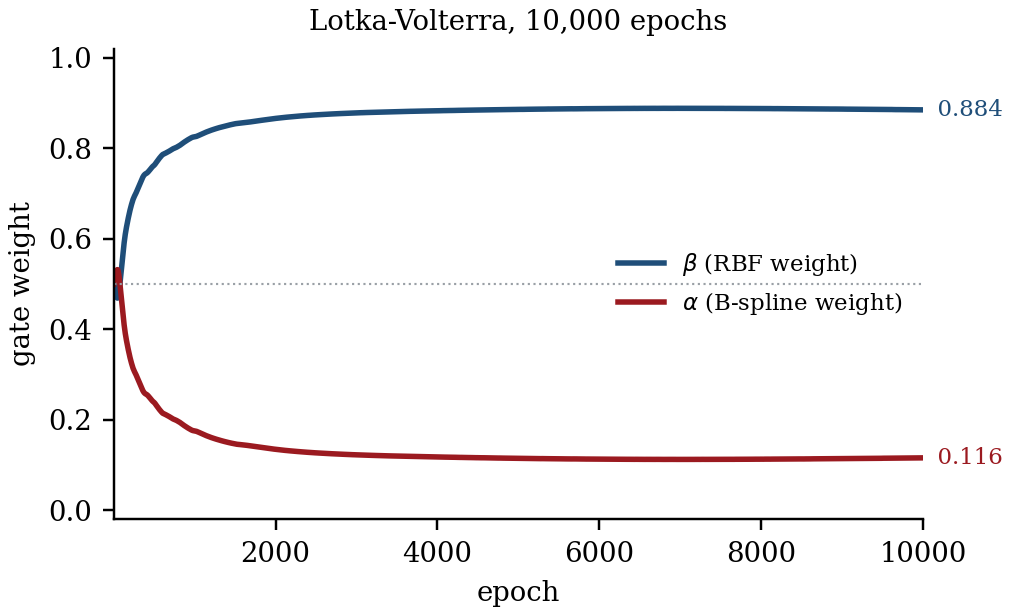
\includegraphics[width=\linewidth]{figures/track_c/lv_full_alpha_beta.png}
\end{minipage}\hfill
\begin{minipage}[t]{0.48\textwidth}
\centering
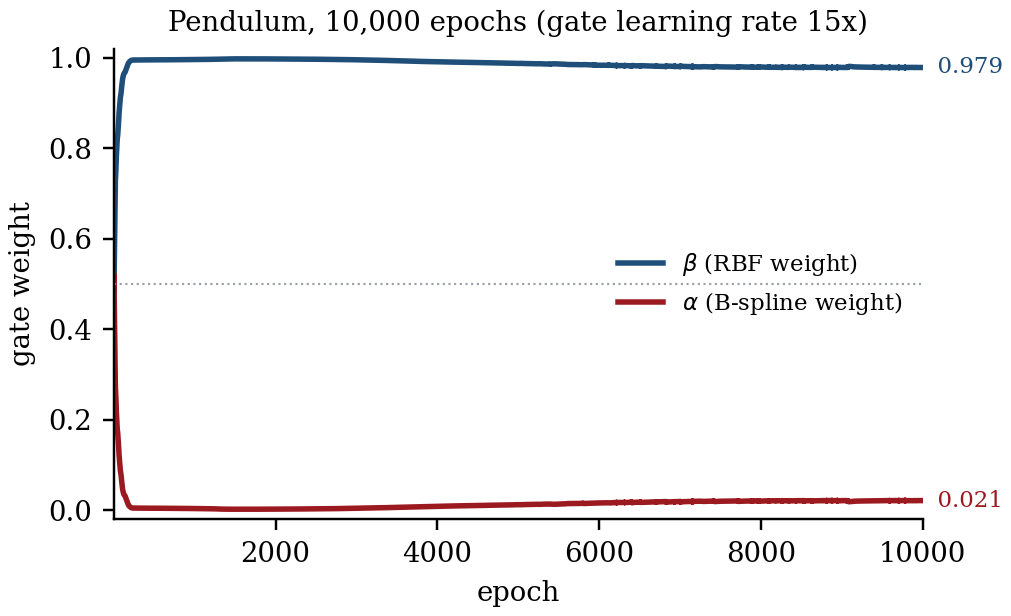
\includegraphics[width=\linewidth]{figures/track_c/pendulum_full_alpha_beta.png}
\end{minipage}
\caption{Learned gate weights over training. Left: Lotka-Volterra settles at
$\alpha=0.116$, $\beta=0.884$. Right: the pendulum gate reaches $\beta=0.995$ by
epoch 250 and peaks at $0.998$ near epoch 1600, then drifts slowly back to
$0.979$ over the rest of the run, the same period in which the model
overfits (discussed below).}
\label{fig:hybrid-gates}
\end{figure}

\paragraph{What the gate does and does not measure.} Because the
coefficients $C$ are shared by both bases and free to grow, the gate is not
identifiable on its own: a small $\alpha$ could in principle be offset by
large coefficients, so the gate value alone does not say how much each basis
contributes. Table~\ref{tab:hybrid-contrib} therefore measures the
contributions directly. It splits each layer's basis output
$C\,(\alpha\,\mathcal B^{\text{spline}}+\beta\,\mathcal B^{\text{RBF}})$ into
its two parts and takes their root-mean-square along the model's own
predicted trajectory. The measured shares track the gate closely, and are
smaller still: the coefficients did not compensate for a small gate weight.

\begin{table}[!ht]
\centering
\footnotesize
\renewcommand{\arraystretch}{1.12}
\caption{Actual contribution of each basis in the trained hybrid models:
root-mean-square of $\alpha\,C\mathcal B^{\text{spline}}$ and
$\beta\,C\mathcal B^{\text{RBF}}$ over the predicted trajectory, per layer,
with the residual path $W\,\mathrm{silu}(x)$ for scale.}
\label{tab:hybrid-contrib}
\begin{tabular}{@{}L{3.6cm} C{1.9cm} C{1.0cm} C{1.7cm} C{1.7cm} C{1.4cm} C{1.6cm}@{}}
\toprule
\hdrrow \thh{Model} & \thh{Gate $(\alpha,\beta)$} & \thh{Layer} & \thh{B-spline part} & \thh{RBF part} & \thh{Residual} & \thh{B-spline share}\\
\midrule
Lotka-Volterra, 10k epochs & $(0.116,\,0.884)$ & 1 & 0.076 & 1.232 & 1.910 & 5.8\%\\
 & & 2 & 0.165 & 2.125 & 2.686 & 7.2\%\\
\addlinespace[2pt]
Pendulum, 3k epochs & $(0.004,\,0.996)$ & 1 & 0.002 & 1.157 & 0.546 & 0.2\%\\
 & & 2 & 0.005 & 2.459 & 1.390 & 0.2\%\\
\addlinespace[2pt]
Pendulum, 10k epochs & $(0.021,\,0.979)$ & 1 & 0.011 & 1.018 & 0.792 & 1.1\%\\
 & & 2 & 0.025 & 2.339 & 1.364 & 1.1\%\\
\bottomrule
\end{tabular}
\end{table}

\paragraph{Lotka-Volterra: no benefit, real cost.} The gate settles at a
partial blend in which the B-spline supplies 6--7\% of the basis output
(Table~\ref{tab:hybrid-contrib}). The hybrid is about $2\times$ worse than
either pure basis on both training MSE ($1.47\times10^{-4}$ against
$8.83\times10^{-5}$ and $7.20\times10^{-5}$) and extrapolation MSE
($1.78\times10^{-4}$ against $8.92\times10^{-5}$ and $8.38\times10^{-5}$;
Table~\ref{tab:hybrid-basis}), while paying roughly the \emph{sum} of their
per-epoch compute. This run used the same learning rate for the gate as for
every other parameter.

\paragraph{Pendulum: overfitting emerges only past a specific budget.} A
short probe run at 2000 epochs first surfaced a practical wrinkle: the gate
moved in the correct direction (toward RBF) but too slowly, so the network
still carried meaningful B-spline contamination at an epoch count where the
pure-RBF pendulum recipe was already nearly converged. Giving the gate its
own, faster learning rate ($15\times$ the base rate, direction untouched)
closed nearly all of that gap at the same probe budget and was carried into
the full pendulum runs (Figure~\ref{fig:hybrid-probe}). The faster gate rate
was applied to the pendulum only; the Lotka-Volterra hybrid above used the
base rate.

\begin{figure}[htbp]
\centering
\begin{minipage}[t]{0.48\textwidth}
\centering
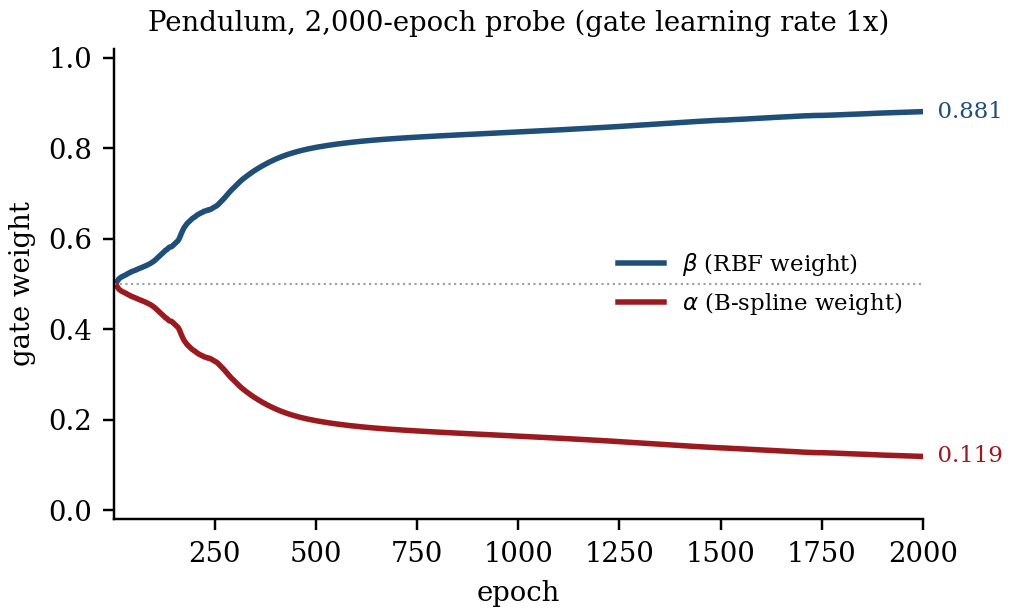
\includegraphics[width=\linewidth]{figures/track_c/hybrid_probe_pendulum_alpha_beta.png}
\end{minipage}\hfill
\begin{minipage}[t]{0.48\textwidth}
\centering
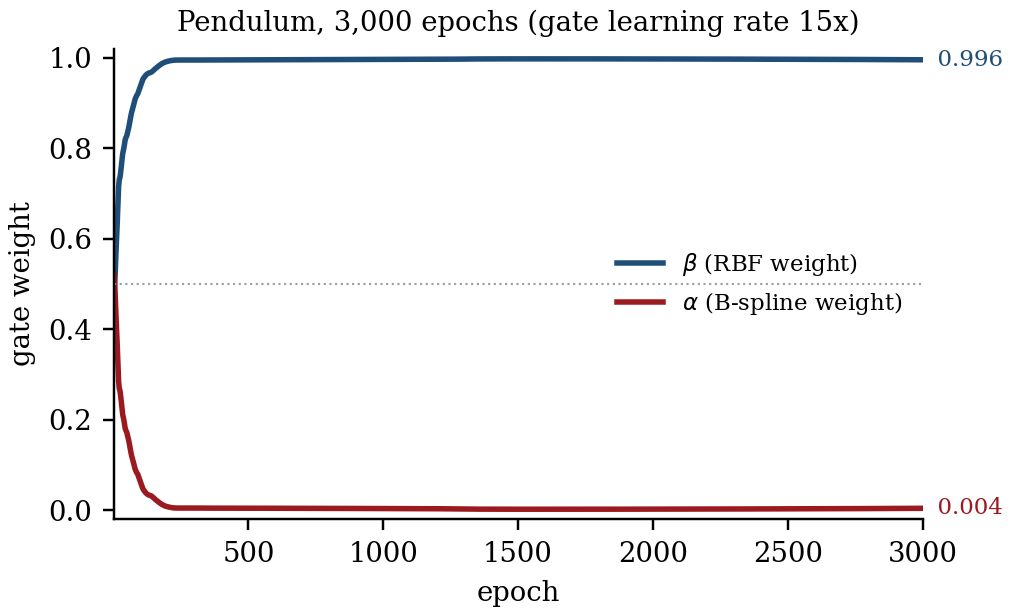
\includegraphics[width=\linewidth]{figures/track_c/hybrid_pendulum_3k_alpha_beta.png}
\end{minipage}
\caption{Left: the 2{,}000-epoch pendulum probe at the base gate learning
rate, whose gate drifts toward RBF only slowly ($\beta=0.881$ at the end),
which motivated the faster gate rate. Right: the 3{,}000-epoch pendulum run
at the faster gate rate discussed below, settling at $\beta=0.996$.}
\label{fig:hybrid-probe}
\end{figure}

At the full 10{,}000-epoch budget, hybrid matches pure RBF's training fit
almost exactly, but its extrapolation collapses ($R^2=-2.17$): the monitor
loss bottoms out near epoch 2950 ($\approx0.054$) then rises to a
$\approx0.4$ plateau for the remaining 7000 epochs while training loss keeps
improving -- textbook overfitting, visible directly in the saved training
history. The gate settles well before this onset: $\beta$ reaches $0.995$ by
epoch 250 (Figure~\ref{fig:hybrid-gates}), and pure RBF trained on the
identical recipe shows no such pattern at all. During the overfitting phase
the gate drifts back from $0.998$ to $0.979$, but the B-spline part still
supplies only 1.1\% of the basis output at the end
(Table~\ref{tab:hybrid-contrib}). So the overfitting cannot be blamed on a
large hidden B-spline contribution. Its cause is not identified here: the
two models differ in their early training path as well as in that small
residual B-spline term.

One further number needs a caveat. Stopping at epoch 3000 gives the hybrid
$0.055$ full-horizon MSE against pure RBF's $0.081$ at the same epoch, with
extrapolation $R^2=+0.580$. That stopping point was chosen from the minimum
of the monitored full-horizon loss, which includes the test window, so it is
an \emph{oracle} early stop that uses test data, which this report's
protocol otherwise forbids (Section~\ref{sec:phase1}). It shows that a good
hybrid model exists along the training path. It does not show that training
could find it without looking at the test window, and it is not counted in
the verdict below.

\begin{keypoint}[Verdict]
Under this report's protocol, where the checkpoint is selected on training
loss, the learnable hybrid basis never outperforms the better pure basis on
either system. On Lotka-Volterra it is about $2\times$ worse than either pure
basis at roughly the sum of their cost. On the pendulum it overfits badly
after about 3000 epochs even though the B-spline supplies only about 1\% of
its basis output. The gate moves in a sensible direction on each system, but
a learned blend buys no accuracy here.
\end{keypoint}

\FloatBarrier
